\section{Tensor Decompositions}\label{chapter:tensor-decomposition}
Working with high-order tensors is computationally expensive because the number of elements grows exponentially with the tensor's order. Tensor decompositions have emerged as powerful and efficient tools to address this issue.
Similar to matrix factorizations, tensor decompositions break down a high-order tensor into smaller components with lower-order and fewer entries, making computations more tractable. However, the notion of the rank of a matrix can be extended in various ways for tensors, each of them associated with a different factorization/decomposition model.
In this chapter, we introduce the most well-known tensor decomposition models.
\subsection{CANDECOMP/PARAFAC~(CP) Decomposition}\label{sec:cp-decomposition}
The CP decomposition~\citep{hitchcock1927expression} of an $N$-th order tensor $\At\in\RR^{d_1\times\cdots\times d_N}$  decomposes $\At$ as the sum of a finite number of rank-one tensors. Equivalently, it is a linear combination of $R$ rank-one tensors where $R$ is called the  rank of the decomposition: 
$$\At = \sum_{r=1}^R \ab^{(r)}_1\outprod\dots\outprod\ab^{(r)}_N ,$$
where $\ab^{(1)}_n,\dots,\ab^{(R)}_n\in\RR^{d_n}$ for each $n\in [N]$.

By grouping all the vectors $\ab^{(r)}_n$ in factor matrices,
\[\Ab_1 = {\begin{pmatrix}
\ab^{(1)}_1 & \dots & \ab^{(R)}_1 \\
\end{pmatrix}}{\in\RR^{d_1\times R}}, \dots ,\Ab_N = {\begin{pmatrix}
\ab^{(1)}_N & \dots & \ab^{(R)}_N \\
\end{pmatrix}}{\in\RR^{d_N\times R}}, \]
the CP decomposition is concisely noted as $\At = \CP{\Ab_1,\cdots,\Ab_N}$.

In tensor networks, a CP decomposition $\At = \CP{\Ab,\Bb,\Cb}$ is represented by
$$
\begin{tikzpicture}[baseline=\baseline]
    \tikzset{tensor/.style = {minimum size = 0.5cm,shape = circle,thick,draw=black,inner sep = 0pt}, edge/.style   = {thick,line width=.4mm},every loop/.style={}}
    \def\y{0}
    \def\x{0}
    \node[tensor,fill=green!50!red!50!white] (A) at (\x,\y){\scalebox{0.85}{$\At$}};
    \draw[edge] (\x+0.25,\y) -- (\x+0.6,\y)  node [midway,above] {\scalebox{0.7}{\dimcolor{$d_2$}}};
    \draw[edge] (\x-0.25,\y) -- (\x-0.6,\y)  node [midway,above] {\scalebox{0.7}{\dimcolor{$d_1$}}};
    \draw[edge] (\x,\y-0.25) -- (\x,\y-0.7)  node [midway,left] {\scalebox{0.7}{\dimcolor{$d_3$}}};
    \end{tikzpicture}
=
\begin{tikzpicture}[baseline=\baseline]
    \tikzset{tensor/.style = {minimum size = 0.5cm,shape = circle,thick,draw=black,inner sep = 0pt}, edge/.style   = {thick,line width=.4mm},every loop/.style={}}
    \def\y{0}
    \def\x{0}
  \node[tensor,fill=red!50!white] (A) at (\x,\y){\scalebox{0.85}{$\Ab$}};
  \node[tensor,fill=blue!50!white] (B) at (\x+1,\y){$\Bb$};
   \node[tensor,fill=blue!20!white] (C) at (\x+2,\y){$\Cb$};
    \draw  node[fill = black,circle,inner sep=0pt,minimum size=4pt] (m) at (\x+1,\y+0.7) {};
    \draw[edge] (A) -- (m);
    \node[draw=none] () at (\x+0.4,\y+0.5) {\scalebox{0.7}{\dimcolor{$R$}}};
    \draw[edge] (B) -- (m) node [midway,left=-0.09cm] {\scalebox{0.7}{\dimcolor{$R$}}};
    \draw[edge] (C) -- (m);
    \node[draw=none] () at (\x+1.6,\y+0.5) {\scalebox{0.7}{\dimcolor{$R$}}};
    \draw[edge](A) -- (\x,\y-0.7)node [midway,left] {\edgelabel{$d_1$}};
    \draw[edge](B) -- (\x+1,\y-0.7)node [midway,left] {\edgelabel{$d_2$}};
    \draw[edge](C) -- (\x+2,\y-0.7)node [midway,left] {\edgelabel{$d_3$}};
\end{tikzpicture},
$$
where the black dot is the third-order copy tensor introduced in Section~\ref{sec:copy-tensor}. Indeed, we have
\begin{align*}
    \left(\begin{tikzpicture}[baseline=\baseline]
    \tikzset{tensor/.style = {minimum size = 0.5cm,shape = circle,thick,draw=black,inner sep = 0pt}, edge/.style   = {thick,line width=.4mm},every loop/.style={}}
    \def\y{0}
    \def\x{0}
  \node[tensor,fill=red!50!white] (A) at (\x,\y){\scalebox{0.85}{$\Ab$}};
  \node[tensor,fill=blue!50!white] (B) at (\x+1,\y){$\Bb$};
   \node[tensor,fill=blue!20!white] (C) at (\x+2,\y){$\Cb$};
    \draw  node[fill = black,circle,inner sep=0pt,minimum size=4pt] (m) at (\x+1,\y+0.7) {};
    \draw[edge] (A) -- (m);
    \node[draw=none] () at (\x+0.4,\y+0.5) {\scalebox{0.7}{\dimcolor{$R$}}};
    \draw[edge] (B) -- (m) node [midway,left=-0.09cm] {\scalebox{0.7}{\dimcolor{$R$}}};
    \draw[edge] (C) -- (m);
    \node[draw=none] () at (\x+1.6,\y+0.5) {\scalebox{0.7}{\dimcolor{$R$}}};
    \draw[edge](A) -- (\x,\y-0.7);
    \draw[edge](B) -- (\x+1,\y-0.7);
    \draw[edge](C) -- (\x+2,\y-0.7);
\end{tikzpicture}\right)_{ijk} 
&= \sum_{r_1=1}^R\sum_{r_2=1}^R\sum_{r_3=1}^R\delta_{r_1r_2r_3}\Ab_{ir_1}\Bb_{jr_2}\Cb_{kr_3}
=
\sum_{r=1}^R\Ab_{ir}\Bb_{jr}\Cb_{kr}\\
&=
\sum_{r=1}^R(\ab_r)_i(\bb_r)_j(\cbb_r)_k 
=
\sum_{r=1}^R(\ab_r\outprod\bb_r\outprod\cbb_r)_{ijk}\\
&=
\left(\sum_{r=1}^R\ab_r\outprod\bb_r\outprod\cbb_r\right)_{ijk}
\end{align*}
\paragraph{CP Rank of a Tensor} 
The most fundamental and oldest concept of the tensor rank is the CP rank, first introduced by~\citep{hitchcock1927expression}. The CP rank of a tensor is defined as the minimum number of rank-one tensors required to express the tensor as their sum.\footnote{Note the subtle difference in our terminology between the rank of a CP decomposition and the CP rank of a tensor:  the rank of a CP decomposition is the number of summands in a decomposition of the form $\At = \sum_{r=1}^R \ab^{(r)}_1\outprod\dots\outprod\ab^{(r)}_N$, whereas the CP rank of a tensor $\At$ is the smallest $R$ for which such a decomposition exists. Consequently, if $\At$ has a rank-$R$ CP decomposition, its CP rank is at most $R$, but could be lower.}
Although this definition is similar to that of matrix rank, the properties of tensor rank differ significantly. From a computational point of view, a key difference is that, unlike matrix rank, there is no polynomial-time algorithm to determine a tensor’s CP rank. In fact, computing the rank of a tensor is an NP-hard problem~\citep{hillar2013most}.
There are several variants of the tensor rank, each associated with a specific tensor decomposition. As we progress through this chapter, we will introduce some of these different types of ranks.


\begin{remark}
\newcommand*{\horzbar}{\rule[.5ex]{2.5ex}{0.5pt}}
We list here some interesting properties of the CP rank and the CP decomposition. 
\begin{enumerate}
\item 
From Theorem~\ref{thm: matricization-rank} and Proposition~\ref{prop:copy.tensor}~(item 3), one can show that if a tensor $\At$ admits a rank-$R$ CP decomposition, then all its matricizations have rank upper bounded by $R$:
\begin{proposition}
    If $\At = \CP{\Ab_1,\cdots, \Ab_N}$ is a rank-$R$ CP decomposition of $\At$, then $\rank(\At_{(I)}) \leq R$ for any $I\subset [N]$.
\end{proposition}
The following tensor network illustrates this result for the matricization of a fourth-order tensor $\At = \CP{\Ab_1,\Ab_2,\Ab_3, \Ab_N}$ along its first two modes.
\begin{align*}
    \left(
    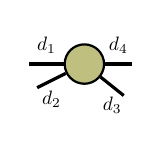
\begin{tikzpicture}[baseline=-0.5ex]
    \tikzset{tensor/.style = {minimum size = 0.5cm,shape = circle,thick,draw=black,inner sep = 0pt}, edge/.style = {thick,line width=.4mm},every loop/.style={}}
    \def\x{6}
    \def\y{0}   \node[tensor,fill=green!50!red!50!white] (T) at (\x+1,\y) {$\At$};
    \draw[edge] (T) -- (\x+0.3,0) node [midway,above] {\scalebox{0.7}{\dimcolor{$d_1$}}};
    \draw[edge] (T) -- (\x+1.6,0) node [midway,above] {\scalebox{0.7}{\dimcolor{$d_4$}}};;
    \draw[edge] (T) -- (\x+0.4,-0.3) node [midway, below] {\scalebox{0.7}{\dimcolor{$d_2$}}};
    \draw[edge] (T) -- (\x+1.5,-0.4)node [midway, below] {\scalebox{0.7}{\dimcolor{$d_3$}}};
\end{tikzpicture}\right)_{(\{1,2\})}
&=
\left(\begin{tikzpicture}[baseline=\baseline]
    \tikzset{tensor/.style = {minimum size = 0.5cm,shape = circle,thick,draw=black,inner sep = 0pt}, edge/.style   = {thick,line width=.4mm},every loop/.style={}}
    \def\y{0}
    \def\x{0}
  \node[tensor,fill=red!50!white] (A) at (\x,\y){\scalebox{0.85}{$\Ab_1$}};
  \node[tensor,fill=blue!50!white] (B) at (\x+1,\y){$\Ab_2$};
   \node[tensor,fill=red!20!white] (C) at (\x+2,\y){$\Ab_3$};
    \node[tensor,fill=blue!20!white] (D) at (\x+3,\y){$\Ab_4$};
    \draw  node[fill = black,circle,inner sep=0pt,minimum size=4pt] (m) at (\x+1.5,\y+0.7) {};
    \draw[edge] (A) -- (m)node [midway, above] {\scalebox{0.7}{\dimcolor{$R$}}} ;
    \draw[edge] (B) -- (m);
    \draw[edge] (C) -- (m);
    \draw[edge] (D) -- (m)node [midway, above] {\scalebox{0.7}{\dimcolor{$R$}}};
    \draw[edge](A) -- (\x,\y-0.7)node [midway,left] {\scalebox{0.7}{\dimcolor{$d_1$}}};
    \draw[edge](B) -- (\x+1,\y-0.7)node [midway,left] {\scalebox{0.7}{\dimcolor{$d_2$}}};
    \draw[edge](C) -- (\x+2,\y-0.7)node [midway,left] {\scalebox{0.7}{\dimcolor{$d_3$}}};
    \draw[edge](D) -- (\x+3,\y-0.7) node [midway,left] {\scalebox{0.7}{\dimcolor{$d_4$}}};
\end{tikzpicture}\right)_{(\{1,2\})}\\
&=
\begin{tikzpicture}[baseline=\baseline]
    \tikzset{tensor/.style = {minimum size = 0.5cm,shape = circle,thick,draw=black,inner sep = 0pt}, edge/.style   = {thick,line width=.4mm},every loop/.style={}}
    \def\y{0}
    \def\x{0}
  \node[tensor,fill=red!50!white] (A) at (\x,\y){\scalebox{0.85}{$\Ab_1$}};
  \node[tensor,fill=blue!50!white] (B) at (\x+1,\y){$\Ab_2$};
   \node[tensor,fill=red!20!white] (C) at (\x+2,\y){$\Ab_3$};
    \node[tensor,fill=blue!20!white] (D) at (\x+3,\y){$\Ab_4$};
    \draw  node[fill = black,circle,inner sep=0pt,minimum size=4pt] (m1) at (\x+0.5,\y+0.7) {};
    \draw  node[fill = black,circle,inner sep=0pt,minimum size=4pt] (m2) at (\x+2.5,\y+0.7) {};
    \draw[edge](A) -- (\x,\y-0.65) -- (\x+0.5,\y-0.65) -- (\x+0.5,\y-1);
    \draw[edge](B) -- (\x+1,\y-0.65) -- (\x+0.6,\y-0.65) -- (\x+0.6,\y-1);
    \draw[edge](C) -- (\x+2,\y-0.65) -- (\x+2.5,\y-0.65) -- (\x+2.5,\y-1);
    \draw[edge](D) -- (\x+3,\y-0.65) -- (\x+2.6,\y-0.65) -- (\x+2.6,\y-1);
    \node[draw=none] at (\x+0.55,\y-1.15){\scalebox{0.7}{\dimcolor{$d_1d_2$}}};
    \node[draw=none] at (\x+2.55,\y-1.15){\scalebox{0.7}{\dimcolor{$d_3d_4$}}};
    \draw[dotted] (\x+1.5,\y+1.5) -- (\x+1.5,\y-0.7);
    \draw[edge](A) -- (m1)node [midway,left] {\scalebox{0.7}{\dimcolor{$R$}}};;
    \draw[edge](B) -- (m1)node [midway,right] {\scalebox{0.7}{\dimcolor{$R$}}};
    \draw[edge](C) -- (m2)node [midway,left] {\scalebox{0.7}{\dimcolor{$R$}}};
    \draw[edge](D) -- (m2)node [midway,right] {\scalebox{0.7}{\dimcolor{$R$}}};
    \draw[edge](m1)--(m2)node [near start, above] {\scalebox{0.7}{\dimcolor{$R$}}};
\end{tikzpicture}.
\end{align*}
\item  The CP rank of a tensor $\At \in \RR^{d_1\times \cdots \times d_N}$ can easily be upper bounded as~\citep{kolda2009tensor}
$$\cprank(\At)\leq \min_{n\in [N]} \prod_{i\neq n} d_i.$$
\item For second-order tensors $\Ab\in\RR^{d_1\times d_2}$, the CP rank corresponds exactly to the classical notion of the rank of a matrix.
\item The CP decomposition $\At = \CP{\Ab,\Bb,\Cb}$ can be expressed using the Kronecker delta 
$$\At_{i,j,k} = \sum_{r_1,r_2,r_3}\delta_{r_1,r_2,r_3}\Ab_{i,r_1}\Bb_{j,r_2}\Cb_{k,r_3},$$
as well as with mode-$n$ products (see~\ref{par:mode-n-tensor-product}) 
$$\At = \It\ttm{1}\Ab\ttm{2}\Bb\ttm{3}\Cb$$
where $\It$ is the third-order copy tensor. 
\item The rank of the second-order tensors (matrices), over the fields $\RR$ and $\CC$ is the same. However, for higher-order tensors ($N$-th order tensors with $N\geq3$) the rank can vary depending on the decomposition field~\citep{kruskal1989rank}.
\item The number of parameters of a CP decomposition of an $N$-th order $d$-dimensional tensors ($d_1 = \dots = d_N = d$) is $NdR$ instead of $d^N$ for the full tensor. If $R$ is small, the number of parameters can be significantly reduced. 
\end{enumerate}
\end{remark}
The following proposition shows how the mode-$n$ matricization of the CP decomposition of a tensor can be expressed using the Khatri-Rao product.
\begin{proposition}
Let $\At\in\RR^{d_1\times d_2\times\dots\times d_N}$. If $\At=\CP{\Ab_1,\Ab_2,\dots,\Ab_N}$, then 
$$\At_{(n)}=\Ab_n\left(\Ab_1\krao\dots\krao\Ab_{(n-1)}\krao\Ab_{(n+1)}\krao\dots\krao\Ab_N\right)^\ts.$$
\begin{proof}
For $N=3$ and $n=1$,
\begin{align*}
\At_{(1)}
&=
\left(\begin{tikzpicture}[baseline=\baseline]
    \tikzset{tensor/.style = {minimum size = 0.5cm,shape = circle,thick,draw=black,inner sep = 0pt}, edge/.style  = {thick,line width=.4mm},every loop/.style={}}
    \def\y{0}
    \def\x{0}
    \node[tensor,fill=green!50!red!50!white] (At) at (\x,\y){\scalebox{0.85}{$\At$}};
    \draw[edge] (\x+0.25,\y) -- (\x+0.6,\y)  node [midway,above] {\scalebox{0.7}{\dimcolor{$d_2$}}};
    \draw[edge] (\x-0.25,\y) -- (\x-0.6,\y)  node [midway,above] {\scalebox{0.7}{\dimcolor{$d_1$}}};
    \draw[edge] (\x,\y-0.25) -- (\x,\y-0.7)  node [midway,left] {\scalebox{0.7}{\dimcolor{$d_3$}}};
    \end{tikzpicture}\right)_{(1)}
=
\left(\begin{tikzpicture}[baseline=\baseline]
    \tikzset{tensor/.style = {minimum size = 0.5cm,shape = circle,thick,draw=black,inner sep = 0pt}, edge/.style   = {thick,line width=.4mm},every loop/.style={}}
    \def\y{0}
    \def\x{0}
  \node[tensor,fill=red!50!white] (A1) at (\x,\y){\scalebox{0.85}{$\Ab_1$}};
  \node[tensor,fill=blue!50!white] (A2) at (\x+1,\y){$\Ab_2$};
   \node[tensor,fill=blue!20!white] (A3) at (\x+2,\y){$\Ab_3$};
    \draw  node[fill = black,circle,inner sep=0pt,minimum size=4pt] (m) at (\x+1,\y+1) {};
    \draw[edge] (A1) -- (m) node [midway,left] {\scalebox{0.7}{\dimcolor{$R$}}};
    \draw[edge] (A2) -- (m)node [midway,left=-0.05cm] {\scalebox{0.7}{\dimcolor{$R$}}};
    \draw[edge] (A3) -- (m)node [midway,right] {\scalebox{0.7}{\dimcolor{$R$}}};
    \draw[edge](A1) -- (\x,\y-0.7)node [midway,left] {\edgelabel{$d_1$}};
    \draw[edge](A2) -- (\x+1,\y-0.7)node [midway,left] {\edgelabel{$d_2$}};
    \draw[edge](A3) -- (\x+2,\y-0.7)node [midway,left] {\edgelabel{$d_3$}};
\end{tikzpicture}\right)_{(1)}\\
&=
\begin{tikzpicture}[baseline=\baseline]
    \tikzset{tensor/.style = {minimum size = 0.5cm,shape = circle,thick,draw=black,inner sep = 0pt}, edge/.style   = {thick,line width=.4mm},every loop/.style={}}
    \def\y{0}
    \def\x{0}
    \node[tensor,fill=green!50!red!50!white] (At) at (\x,\y){\scalebox{0.85}{$\At$}};
    \draw[edge] (\x-0.25,\y) -- (\x-0.6,\y)  node [midway,above] {\scalebox{0.7}{\dimcolor{$d_1$}}};
    \draw[edge] (\x+0.2,\y+0.15) -- (\x+0.5,\y+0.15)-- (\x+0.5,\y+0.05) -- (\x+1,\y+0.05) node [midway,above]
    {\scalebox{0.7}{\dimcolor{$d_2$}}};
    \draw[edge] (\x+0.2,\y-0.15) -- (\x+0.5,\y-0.15)-- (\x+0.5,\y-0.05)-- (\x+1,\y-0.05) node [midway,below]
    {\scalebox{0.7}{\dimcolor{$d_3$}}};
    \end{tikzpicture}
=
\begin{tikzpicture}[baseline=\baseline]
    \tikzset{tensor/.style = {minimum size = 0.5cm,shape = circle,thick,draw=black,inner sep = 0pt}, edge/.style   = {thick,line width=.4mm},every loop/.style={}}
    \def\y{0}
    \def\x{0}
    \node[tensor,fill=red!50!white] (A1) at (\x,\y){\scalebox{0.85}{$\Ab_1$}};
    \node[tensor,fill=blue!50!white] (A2) at (\x+1.7,\y+0.7){$\Ab_2$};
    \node[tensor,fill=blue!20!white] (A3) at (\x+1.7,\y-0.7){$\Ab_3$};
    \draw  node[fill = black,circle,inner sep=0pt,minimum size=4pt] (m) at (\x+1,\y) {};
    \draw[edge] (A1) -- (m) node [very near end,above] {\scalebox{0.7}{\dimcolor{$R$}}};
    \draw[edge] (A2) -- (m);
    \draw[edge] (A3) -- (m);
    \draw[edge] (A1) -- (\x-0.7,\y) node [midway,above] {\scalebox{0.7}{\dimcolor{$d_1$}}};
    \draw[edge] (A2) -- (\x+2.5,\y+0.7) -- (\x+2.5,\y+0.05)-- (\x+3,\y+0.05) node [midway,above]
    {\scalebox{0.7}{\dimcolor{$d_2$}}};
    \draw[edge] (A3) -- (\x+2.5,\y-0.7) -- (\x+2.5,\y-0.05) -- (\x+3,\y-0.05) node [midway,below]
    {\scalebox{0.7}{\dimcolor{$d_3$}}};
    \end{tikzpicture}
=
\Ab_1(\Ab_2\krao\Ab_3)^\ts.
\end{align*}
\end{proof}
\end{proposition}

